\documentclass{article}

\usepackage{fancyhdr}
\usepackage{extramarks}
\usepackage{amsmath}
\usepackage{amsthm}
\usepackage{amsfonts}
\usepackage{tikz}
\usepackage[plain]{algorithm}
\usepackage{algpseudocode}
\usepackage{graphicx}

\graphicspath{{./images/}}

\usetikzlibrary{automata,positioning}

%
% Basic Document Settings
%

\topmargin=-0.45in
\evensidemargin=0in
\oddsidemargin=0in
\textwidth=6.5in
\textheight=9.0in
\headsep=0.25in

\linespread{1.1}

\pagestyle{fancy}
\lhead{\hmwkAuthorName}
\chead{\hmwkClass\ \hmwkTitle}
\rhead{\firstxmark}
\lfoot{\lastxmark}
\cfoot{\thepage}

\renewcommand\headrulewidth{0.4pt}
\renewcommand\footrulewidth{0.4pt}

\setlength\parindent{0pt}

%
% Create Problem Sections
%

\newcommand{\enterProblemHeader}[1]{
    \nobreak\extramarks{}{Problem {#1} continued on next page\ldots}\nobreak{}
    \nobreak\extramarks{Problem {#1} (continued)}{Problem {#1} continued on next page\ldots}\nobreak{}
}

\newcommand{\exitProblemHeader}[1]{
    \nobreak\extramarks{Problem {#1} (continued)}{Problem {#1} continued on next page\ldots}\nobreak{}
    % \stepcounter{#1}
    \nobreak\extramarks{Problem {#1}}{}\nobreak{}
}

\setcounter{secnumdepth}{0}
\newcounter{partCounter}

\newcommand{\problemNumber}{0.0}

\newenvironment{homeworkProblem}[1][-1]{
    \renewcommand{\problemNumber}{{#1}}
    \section{Problem \problemNumber}
    \setcounter{partCounter}{1}
    \enterProblemHeader{\problemNumber}
}{
    \exitProblemHeader{\problemNumber}
}

%
% Homework Details
%   - Title
%   - Class
%   - Author
%

\newcommand{\hmwkTitle}{Homework\ \#2}
\newcommand{\hmwkClass}{RBE 500}
\newcommand{\hmwkAuthorName}{\textbf{Arjan Gupta}}

%
% Title Page
%

\title{
    \vspace{2in}
    \textmd{\textbf{\hmwkClass\ \hmwkTitle}}\\
    \vspace{3in}
}

\author{\hmwkAuthorName}
\date{}

\renewcommand{\part}[1]{\textbf{\large Part \Alph{partCounter}}\stepcounter{partCounter}\\}

%
% Various Helper Commands
%

% Useful for algorithms
\newcommand{\alg}[1]{\textsc{\bfseries \footnotesize #1}}

% For derivatives
\newcommand{\deriv}[1]{\frac{\mathrm{d}}{\mathrm{d}x} (#1)}

% For partial derivatives
\newcommand{\pderiv}[2]{\frac{\partial}{\partial #1} (#2)}

% Integral dx
\newcommand{\dx}{\mathrm{d}x}

% Alias for the Solution section header
\newcommand{\solution}{\textbf{\large Solution}}

% Probability commands: Expectation, Variance, Covariance, Bias
\newcommand{\E}{\mathrm{E}}
\newcommand{\Var}{\mathrm{Var}}
\newcommand{\Cov}{\mathrm{Cov}}
\newcommand{\Bias}{\mathrm{Bias}}

\begin{document}

\maketitle

\nobreak\extramarks{Problem 3.5}{}\nobreak{}

\pagebreak

\begin{homeworkProblem}[3.5]
    Consider the three-link articulated robot of Figure 3.16. Derive the forward kinematic equations using the DH convention.
    \begin{figure}[h]
        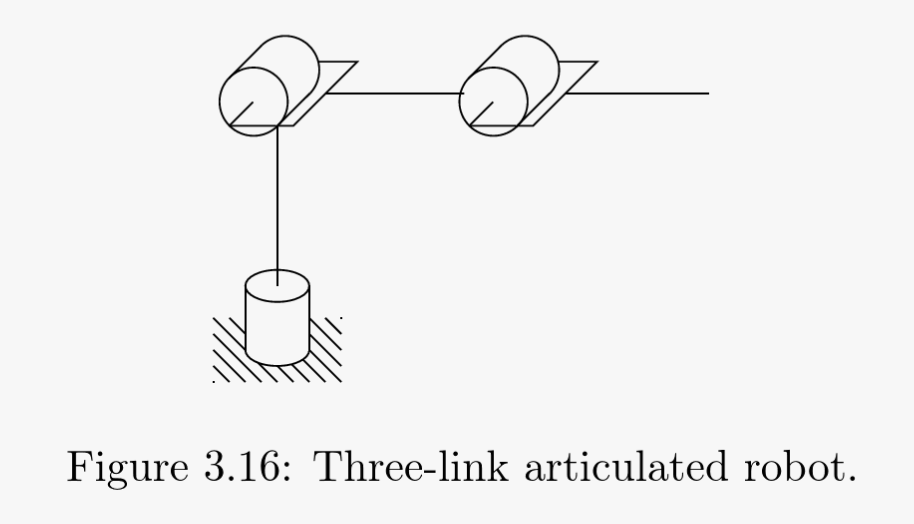
\includegraphics[scale=0.25]{figure3-16.png}
        \centering
    \end{figure}

    \textbf{Solution}
    \vspace{0.1in}\\
    First we assign coordinate frames 0 through 3 (links 0 through 3). This is done as per the following figure.
    \begin{figure}[h]
        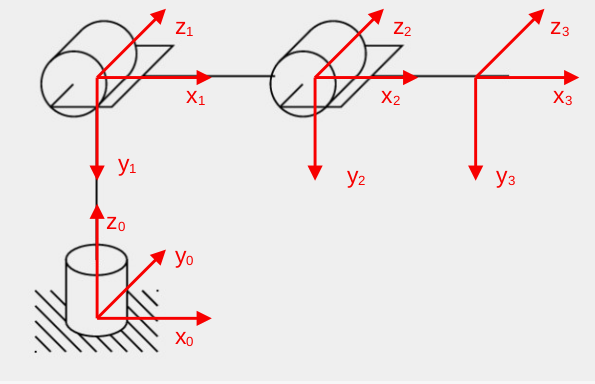
\includegraphics[scale=0.4]{problem-3-5-figure-frames.png}
        \centering
    \end{figure}

    Now, we create a table for quantities \(\alpha_i, a_i, \theta_i, d_i\) for links 1 through 3.

    \begin{table}[h!]
        \begin{center}
            \caption{Your first table.}\label{tab:table1}
            \begin{tabular}{c|c|c} % <-- Alignments: 1st column left, 2nd middle and 3rd right, with vertical lines in between
            $\alpha$ & $\beta$ & $\gamma$ \\
            \hline
            1 & 1110.1 & a\\
            2 & 10.1 & b\\
            3 & 23.113231 & c\\
            \end{tabular}
        \end{center}
    \end{table}

\end{homeworkProblem}

\pagebreak

\begin{homeworkProblem}
    Let \(\Sigma = \{0, 1\}\). Construct a DFA \(A\) that recognizes the
    language that consists of all binary numbers that can be divided by 5.
    vspace
    \\
    Let the state \(q_k\) indicate the remainder of \(k\) divided by 5. For
    example, the remainder of 2 would correlate to state \(q_2\) because \(7
    \mod 5 = 2\).

    \begin{figure}[h]
        \centering
        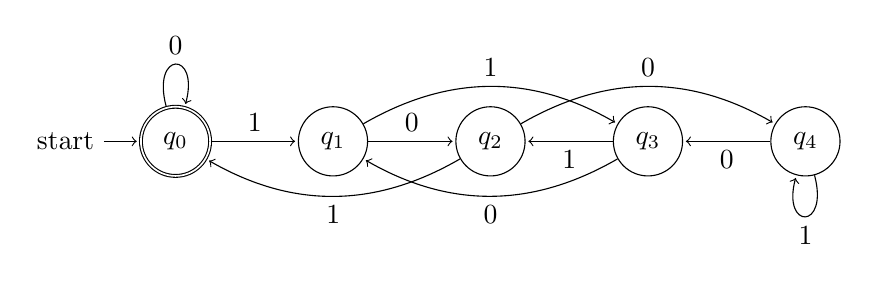
\begin{tikzpicture}[shorten >=1pt,node distance=2cm,on grid,auto]
            \node[state, accepting, initial] (q_0)   {$q_0$};
            \node[state] (q_1) [right=of q_0] {$q_1$};
            \node[state] (q_2) [right=of q_1] {$q_2$};
            \node[state] (q_3) [right=of q_2] {$q_3$};
            \node[state] (q_4) [right=of q_3] {$q_4$};
            \path[->]
                (q_0)
                    edge [loop above] node {0} (q_0)
                    edge node {1} (q_1)
                (q_1)
                    edge node {0} (q_2)
                    edge [bend right=-30] node {1} (q_3)
                (q_2)
                    edge [bend left] node {1} (q_0)
                    edge [bend right=-30] node {0} (q_4)
                (q_3)
                    edge node {1} (q_2)
                    edge [bend left] node {0} (q_1)
                (q_4)
                    edge node {0} (q_3)
                    edge [loop below] node {1} (q_4);
        \end{tikzpicture}
        \caption{DFA, \(A\), this is really beautiful, ya know?}
        \label{fig:multiple5}
    \end{figure}

    \textbf{Justification}
    \\

    Take a given binary number, \(x\). Since there are only two inputs to our
    state machine, \(x\) can either become \(x0\) or \(x1\). When a 0 comes
    into the state machine, it is the same as taking the binary number and
    multiplying it by two. When a 1 comes into the machine, it is the same as
    multipying by two and adding one.
    \\

    Using this knowledge, we can construct a transition table that tell us
    where to go:

    \begin{table}[ht]
        \centering
        \begin{tabular}{c || c | c | c | c | c}
            & \(x \mod 5 = 0\)
            & \(x \mod 5 = 1\)
            & \(x \mod 5 = 2\)
            & \(x \mod 5 = 3\)
            & \(x \mod 5 = 4\)
            \\
            \hline
            \(x0\) & 0 & 2 & 4 & 1 & 3 \\
            \(x1\) & 1 & 3 & 0 & 2 & 4 \\
        \end{tabular}
    \end{table}

    Therefore on state \(q_0\) or (\(x \mod 5 = 0\)), a transition line should
    go to state \(q_0\) for the input 0 and a line should go to state \(q_1\)
    for input 1. Continuing this gives us the Figure~\ref{fig:multiple5}.
\end{homeworkProblem}

\begin{homeworkProblem}
    Write part of \alg{Quick-Sort($list, start, end$)}

    \begin{algorithm}[]
        \begin{algorithmic}[1]
            \Function{Quick-Sort}{$list, start, end$}
                \If{$start \geq end$}
                    \State{} \Return{}
                \EndIf{}
                \State{} $mid \gets \Call{Partition}{list, start, end}$
                \State{} \Call{Quick-Sort}{$list, start, mid - 1$}
                \State{} \Call{Quick-Sort}{$list, mid + 1, end$}
            \EndFunction{}
        \end{algorithmic}
        \caption{Start of QuickSort}
    \end{algorithm}
\end{homeworkProblem}

\pagebreak

\begin{homeworkProblem}
    Suppose we would like to fit a straight line through the origin, i.e.,
    \(Y_i = \beta_1 x_i + e_i\) with \(i = 1, \ldots, n\), \(\E [e_i] = 0\),
    and \(\Var [e_i] = \sigma^2_e\) and \(\Cov[e_i, e_j] = 0, \forall i \neq
    j\).\\
    \part

    Find the least squares esimator for \(\hat{\beta_1}\) for the slope
    \(\beta_1\).
    \\

    \solution

    To find the least squares estimator, we should minimize our Residual Sum
    of Squares, RSS:

    \[
        \begin{split}
            RSS &= \sum_{i = 1}^{n} {(Y_i - \hat{Y_i})}^2
            \\
            &= \sum_{i = 1}^{n} {(Y_i - \hat{\beta_1} x_i)}^2
        \end{split}
    \]

    By taking the partial derivative in respect to \(\hat{\beta_1}\), we get:

    \[
        \pderiv{
            \hat{\beta_1}
        }{RSS}
        = -2 \sum_{i = 1}^{n} {x_i (Y_i - \hat{\beta_1} x_i)}
        = 0
    \]

    This gives us:

    \[
        \begin{split}
            \sum_{i = 1}^{n} {x_i (Y_i - \hat{\beta_1} x_i)}
            &= \sum_{i = 1}^{n} {x_i Y_i} - \sum_{i = 1}^{n} \hat{\beta_1} x_i^2
            \\
            &= \sum_{i = 1}^{n} {x_i Y_i} - \hat{\beta_1}\sum_{i = 1}^{n} x_i^2
        \end{split}
    \]

    Solving for \(\hat{\beta_1}\) gives the final estimator for \(\beta_1\):

    \[
        \begin{split}
            \hat{\beta_1}
            &= \frac{
                \sum {x_i Y_i}
            }{
                \sum x_i^2
            }
        \end{split}
    \]

    \pagebreak

    \part

    Calculate the bias and the variance for the estimated slope
    \(\hat{\beta_1}\).
    \\

    \solution

    For the bias, we need to calculate the expected value
    \(\E[\hat{\beta_1}]\):

    \[
        \begin{split}
            \E[\hat{\beta_1}]
            &= \E \left[ \frac{
                \sum {x_i Y_i}
            }{
                \sum x_i^2
            }\right]
            \\
            &= \frac{
                \sum {x_i \E[Y_i]}
            }{
                \sum x_i^2
            }
            \\
            &= \frac{
                \sum {x_i (\beta_1 x_i)}
            }{
                \sum x_i^2
            }
            \\
            &= \frac{
                \sum {x_i^2 \beta_1}
            }{
                \sum x_i^2
            }
            \\
            &= \beta_1 \frac{
                \sum {x_i^2 \beta_1}
            }{
                \sum x_i^2
            }
            \\
            &= \beta_1
        \end{split}
    \]

    Thus since our estimator's expected value is \(\beta_1\), we can conclude
    that the bias of our estimator is 0.
    \\

    For the variance:

    \[
        \begin{split}
            \Var[\hat{\beta_1}]
            &= \Var \left[ \frac{
                \sum {x_i Y_i}
            }{
                \sum x_i^2
            }\right]
            \\
            &=
            \frac{
                \sum {x_i^2}
            }{
                \sum x_i^2 \sum x_i^2
            } \Var[Y_i]
            \\
            &=
            \frac{
                \sum {x_i^2}
            }{
                \sum x_i^2 \sum x_i^2
            } \Var[Y_i]
            \\
            &=
            \frac{
                1
            }{
                \sum x_i^2
            } \Var[Y_i]
            \\
            &=
            \frac{
                1
            }{
                \sum x_i^2
            } \sigma^2
            \\
            &=
            \frac{
                \sigma^2
            }{
                \sum x_i^2
            }
        \end{split}
    \]

\end{homeworkProblem}

\pagebreak

\begin{homeworkProblem}
    Prove a polynomial of degree \(k\), \(a_kn^k + a_{k - 1}n^{k - 1} + \hdots
    + a_1n^1 + a_0n^0\) is a member of \(\Theta(n^k)\) where \(a_k \hdots a_0\)
    are nonnegative constants.

    \begin{proof}
        To prove that \(a_kn^k + a_{k - 1}n^{k - 1} + \hdots + a_1n^1 +
        a_0n^0\), we must show the following:

        \[
            \exists c_1 \exists c_2 \forall n \geq n_0,\ {c_1 \cdot g(n) \leq
            f(n) \leq c_2 \cdot g(n)}
        \]

        For the first inequality, it is easy to see that it holds because no
        matter what the constants are, \(n^k \leq a_kn^k + a_{k - 1}n^{k - 1} +
        \hdots + a_1n^1 + a_0n^0\) even if \(c_1 = 1\) and \(n_0 = 1\).  This
        is because \(n^k \leq c_1 \cdot a_kn^k\) for any nonnegative constant,
        \(c_1\) and \(a_k\).
        \\

        Taking the second inequality, we prove it in the following way.
        By summation, \(\sum\limits_{i=0}^k a_i\) will give us a new constant,
        \(A\). By taking this value of \(A\), we can then do the following:

        \[
            \begin{split}
                a_kn^k + a_{k - 1}n^{k - 1} + \hdots + a_1n^1 + a_0n^0 &=
                \\
                &\leq (a_k + a_{k - 1} \hdots a_1 + a_0) \cdot n^k
                \\
                &= A \cdot n^k
                \\
                &\leq c_2 \cdot n^k
            \end{split}
        \]

        where \(n_0 = 1\) and \(c_2 = A\). \(c_2\) is just a constant. Thus the
        proof is complete.
    \end{proof}
\end{homeworkProblem}

\pagebreak

%
% Non sequential homework problems
%

% Jump to problem 18
\begin{homeworkProblem}[18]
    Evaluate \(\sum_{k=1}^{5} k^2\) and \(\sum_{k=1}^{5} (k - 1)^2\).
\end{homeworkProblem}

% Continue counting to 19
\begin{homeworkProblem}
    Find the derivative of \(f(x) = x^4 + 3x^2 - 2\)
\end{homeworkProblem}

% Go back to where we left off
\begin{homeworkProblem}[6]
    Evaluate the integrals
    \(\int_0^1 (1 - x^2) \dx\)
    and
    \(\int_1^{\infty} \frac{1}{x^2} \dx\).
\end{homeworkProblem}

\end{document}